\chapter{Methodology}
\label{chap:methodology}

This chapter sets out how the research was conducted, in three parts: the
\emph{research method} (\refsec{sec:m-design}); the \emph{development} of the artefact
the experiments run on (\refsec{sec:m-dev}) and the technical detail of each component
(\refsec{sec:m-env}--\refsec{sec:m-train}); and the \emph{experimentation}
(\refsec{sec:m-experiments}, \refsec{sec:m-eval}).

The pipeline that results is summarised in \reffig{fig:pipeline}. The
methodological principle throughout is a strict
separation of roles: the scripted expert \emph{teaches} by producing clean
demonstrations, but at inference the neural policy is in sole control of the
robot, receiving only images, proprioception and the language instruction.

\begin{figure}[ht]
\begin{center}
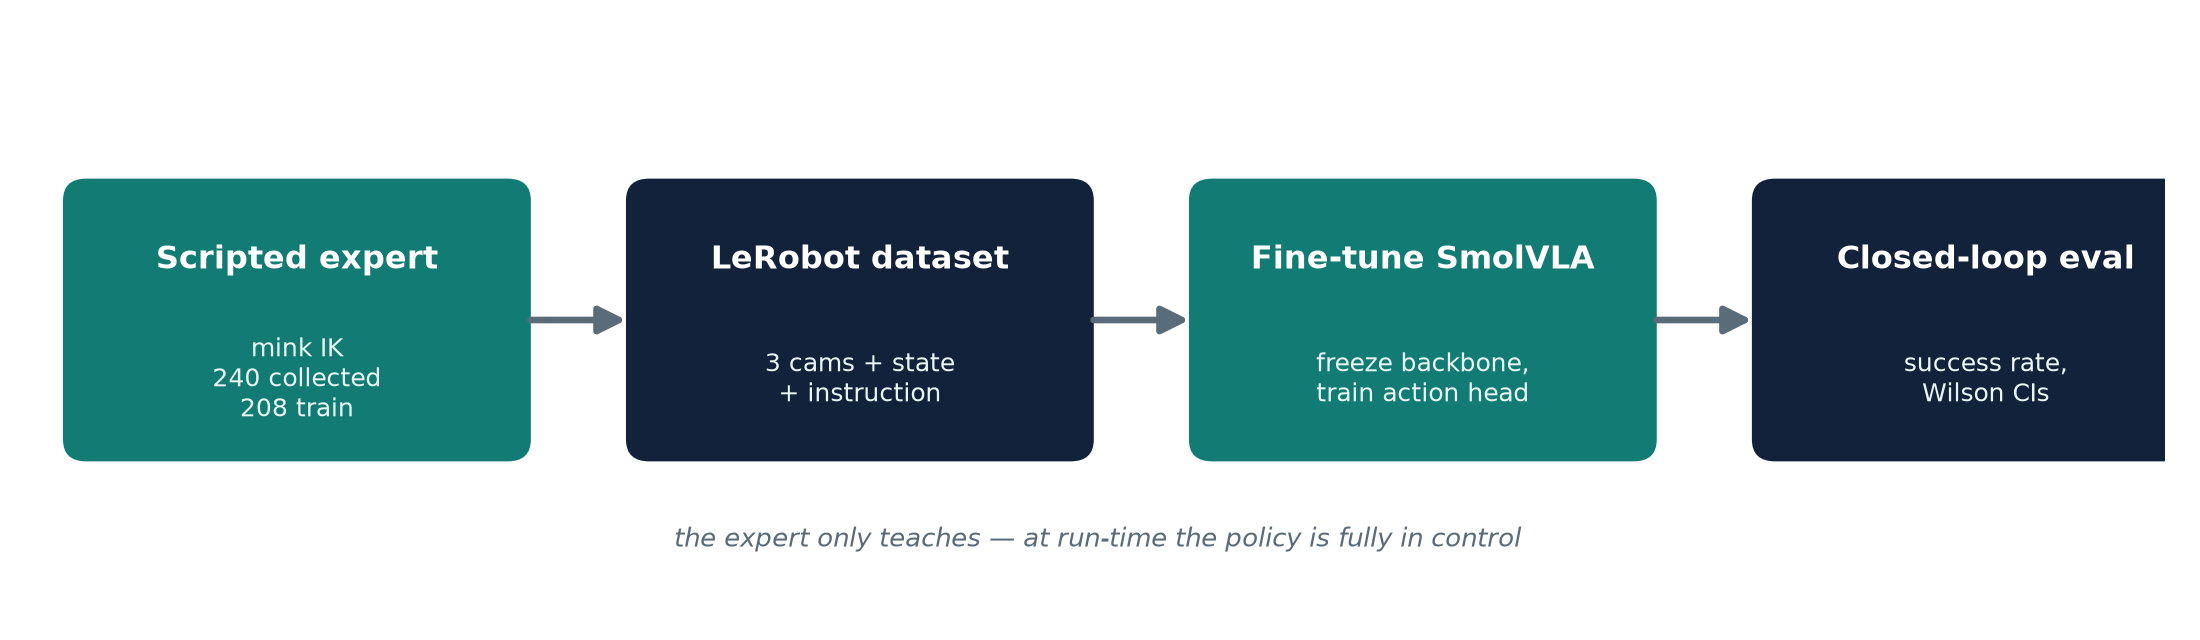
\includegraphics[width=\textwidth,
    alt={A four-stage pipeline: scripted expert with mink inverse kinematics generating 208 training demonstrations, a LeRobot dataset of three cameras plus state plus instruction, fine-tuning SmolVLA with a frozen backbone, and closed-loop evaluation with Wilson confidence intervals.}]{figures/fig_pipeline}
\end{center}
\caption{The experimental pipeline. A scripted inverse-kinematics expert generates
demonstrations, which are converted to the LeRobot dataset format and used to
fine-tune SmolVLA (backbone frozen, action expert trained); the policy is then
evaluated closed-loop.}
\label{fig:pipeline}
\end{figure}

\section{Research design}
\label{sec:m-design}

\subsection{Research strategy}
\label{sec:m-strategy}
The work is an \emph{empirical, quantitative} study in the hypothetico-deductive mode:
each research question of \refsec{sec:rqs} becomes a prediction a controlled experiment
can confirm or refute, run at a sample size chosen so the outcome is informative rather
than anecdotal. Evidence is numerical --- success rates over many closed-loop rollouts
with interval estimates --- supplemented by qualitative tracing where a number alone
does not identify a cause (\refsec{sec:results-diagnosis}).

It combines two activities usually kept apart: \emph{construction}, since no
off-the-shelf environment, expert or dataset existed; and \emph{controlled
experimentation} on the artefact so constructed. This is design-oriented engineering
research, in which an artefact is built to make a phenomenon observable and the
knowledge claim rests on what is measured. Artefact and findings therefore developed
together, and the build history is reported rather than tidied away
(\refsec{sec:m-dev}, \refsec{sec:results-journey}).

Because the artefact was built by the same person who evaluates it, the design separates
the two roles wherever it can: success is defined geometrically and scored by code, not
by inspection; the identical criterion gates collection and evaluation, so the
definition cannot drift; evaluation is automated end to end; and the deployment
checkpoint is chosen by a pre-declared rule. Where a claim rests on judgement, this is
stated.

\subsection{Why simulation}
\label{sec:m-whysim}
The entire study is conducted in the MuJoCo physics simulator
\parencite{todorov2012mujoco}. This is a methodological choice, not merely a
practical one, and it is justified on four grounds.

\begin{enumerate}
    \item \textbf{Statistical power.} The conclusions rest on more than 1{,}300
    closed-loop rollouts (\reftab{tab:experiments}) --- not attainable on hardware
    within an MSc project, but a few days of headless compute in simulation. Since
    \refsec{sec:bg-eval} identifies under-powered evaluation as the dominant hazard in
    this literature, a setting that makes adequate samples affordable answers it
    directly.
    \item \textbf{Ground truth.} The displacement experiment of
    \refsec{sec:results-lookup} needs the exact pose of every object and of the gripper
    at closure, and objects placed at prescribed positions repeatably to the
    millimetre --- free in simulation, and requiring motion capture on hardware.
    \item \textbf{Control of confounds.} Testing whether a policy localises the named
    item or recalls its position requires holding everything constant except object
    position, including the random seed.
    \item \textbf{Cost and safety.} No hardware was available under the project's
    budget, and a \SI{1.3}{m}-reach industrial arm running an unvalidated learned
    policy would require a safety case disproportionate to the question asked.
\end{enumerate}

The limitation is stated plainly: no claim of sim-to-real transfer is made, no domain
randomisation is employed, and the reality gap of \refsec{sec:bg-sim} applies in full.
To keep a later transfer study possible, the pipeline uses tooling a real-robot study
would also use --- LeRobot \parencite{cadene2024lerobot} and manufacturer-derived models
of a real arm, gripper and base.

\subsection{Phased structure of the study}
\label{sec:m-phases}
The research proceeded in three phases (\reftab{tab:phases-study}). Each ended in an
empirical result that determined the next, and they are reported in that order in
\refChap{chap:results} rather than as a single pre-planned design, because the
reasoning from one to the next is part of the contribution.

\begin{table}[ht]
\caption{The three phases of the study. Each phase terminated in a result that
determined the scope of the next.}
\begin{center}
\tagpdfsetup{table/header-rows={1}}
\begin{tabular}{p{0.13\textwidth}p{0.24\textwidth}p{0.24\textwidth}p{0.27\textwidth}}
\toprule
Phase & Setting & Question & Outcome that set the next phase \\
\midrule
1. Benchmark feasibility &
RoboCasa kitchen benchmark, Franka on a mobile base &
Can deployable small models perform an established benchmark after task-specific
fine-tuning? &
No: 0/20 for both SmolVLA and ACT. Difficulty had to be reduced along every axis at
once. \\
\addlinespace
2. Controlled pilot &
Fixed-base UR10e, single cube, five positions &
Can the same small models learn a controlled task, and what dominates performance? &
Yes ($\sim$47--53\%), but a metric bug, duplicated data and a memory ceiling
mattered more than model choice. \\
\addlinespace
3. Main study &
Simulated supermarket: UR10e on an Omron base, four grocery items, language-conditioned &
What can a compact VLA do under a \SI{12}{GB} ceiling, and what has it actually
learned? &
Reported in full in \refChap{chap:results}. \\
\bottomrule
\end{tabular}
\end{center}
\label{tab:phases-study}
\end{table}

The narrowing follows \refsec{sec:bg-sim}'s diagnosis of \emph{why} RoboCasa is hard
for a small model. Phase 2 removed all four compounding difficulties at once; Phase 3
reintroduced the task-relevant complexity while retaining experimental control. Phases 1
and 2 are reported in \refsec{sec:results-journey}; the remainder of this chapter
describes Phase 3.

\subsection{From research questions to experiments}
\label{sec:m-rq-map}
\reftab{tab:rqmap} maps each research question onto the experiments that answer it
and the measurement each yields. The catalogue of experiments itself, with sample
sizes and conditions, is given in \refsec{sec:m-experiments}.

\begin{table}[ht]
\caption{Mapping from research questions (\refsec{sec:rqs}) to experiments and
measurements. Experiment identifiers refer to \reftab{tab:experiments}.}
\begin{center}
\tagpdfsetup{table/header-rows={1}}
\begin{tabular}{p{0.09\textwidth}p{0.36\textwidth}p{0.11\textwidth}p{0.32\textwidth}}
\toprule
RQ & Prediction to be tested & Experiments & Measurement \\
\midrule
RQ1 & A compact VLA fine-tuned within \SI{12}{GB} completes the task more often than
not. & E3, E7 & Task-completion rate with Wilson interval; peak GPU memory. \\
\addlinespace
RQ2 & At this scale, changes to data, metrics and observability move performance more
than changes to model capacity. & E1, E2, E4, E8 & Success rate before and after each
intervention; same-task comparison against a policy $1/8$ the size. \\
\addlinespace
RQ3 & If the policy is language-conditioned, the reach follows the instruction; if it
is \emph{visually grounded}, the reach follows the object when the two are decoupled.
& E5, E6, E7 & Gripper lateral position at gripper closure versus actual and versus
trained item position. \\
\addlinespace
RQ4 & The failure is localisable to one stage of the
perception--language--grasp--place chain and correctable without adding capacity. &
E4, E6 & Per-stage outcome (grasp versus placement); success rate after each targeted
change. \\
\bottomrule
\end{tabular}
\end{center}
\label{tab:rqmap}
\end{table}

\section{Development methodology}
\label{sec:m-dev}
The artefact was developed \emph{iteratively and incrementally}: as a sequence of
small, independently runnable stages, each with its own verification, so a defect could
be attributed to a stage rather than to the system as a whole. This matters because the
thesis's central methodological claim --- that diagnosis outperforms scaling --- is
only actionable if failures can be localised.

\subsection{Increments and their acceptance criteria}
\label{sec:m-increments}
\reftab{tab:increments} lists the increments in order with the check that had to pass
before the next began. Every increment is verified against a criterion that does
\emph{not} depend on the learned policy, so when a policy later fails, the stages
beneath it are already validated.

\begin{table}[ht]
\caption{Development increments and the acceptance check applied to each before
proceeding. Each check is independent of the learned policy.}
\begin{center}
\tagpdfsetup{table/header-rows={1}}
\begin{tabular}{p{0.05\textwidth}p{0.30\textwidth}p{0.55\textwidth}}
\toprule
\# & Increment & Acceptance check \\
\midrule
1 & Scene model: base, arm, gripper, shelf, products, cameras &
Arm converges to commanded joint targets under gravity compensation; products rest
stably; all three cameras render headlessly through EGL. \\
\addlinespace
2 & Inverse-kinematics solver for grasp and place poses &
Solutions lie on the kinematic branch the position servos can track, seeded from the
home configuration; no joint wrapping beyond $\pm 2\pi$. \\
\addlinespace
3 & Scripted expert trajectory &
Per-item success under per-episode jitter measured over repeated runs
(\reftab{tab:grasptune}); items with unreliable expert performance excluded rather
than carried into the dataset. \\
\addlinespace
4 & Demonstration recorder and dataset conversion &
Every retained episode passes the \emph{same} geometric placement check later used to
score the policy; frame counts, camera streams, state/action dimensions and
instruction labels verified on the converted dataset. \\
\addlinespace
5 & Fine-tuning configuration &
Training completes within the \SI{12}{GB} budget with peak memory recorded; loss
decreases; checkpoints written at fixed intervals. \\
\addlinespace
6 & Closed-loop evaluation harness &
Scripted expert scored through the harness reproduces its known success rate,
confirming the harness measures what it claims to; normalisation statistics loaded
from the checkpoint under test. \\
\addlinespace
7 & Multi-item orchestrator &
Arm returns to the in-distribution home configuration between items; basket contents
persist across picks; retry logic disabled for measurement runs. \\
\bottomrule
\end{tabular}
\end{center}
\label{tab:increments}
\end{table}

\subsection{The diagnostic loop}
\label{sec:m-diagnostic-loop}
Where a trained policy underperformed, the response followed a fixed rule, adopted
after the Phase-2 experience described in \refsec{sec:results-journey}:

\begin{enumerate}
    \item \textbf{Reproduce and instrument} the failure over enough trials to
    establish that it is systematic rather than sampling noise.
    \item \textbf{Trace a single episode} frame by frame, recording object and
    gripper poses, to establish \emph{where} in the perception--language--grasp--place
    chain the behaviour departs from the demonstration.
    \item \textbf{Form a mechanism hypothesis} that predicts something not yet
    measured.
    \item \textbf{Change one thing} that the hypothesis implicates --- the data, the
    observation, or the environment --- and re-measure under the identical protocol.
    \item \textbf{Only then consider capacity.} Increasing model size, training
    steps or dataset volume was treated as the last resort, not the first.
\end{enumerate}

This rule produced the sequence in \refsec{sec:results-diagnosis}, and also the most
uncomfortable result in the thesis: applying step~3 to an apparently successful
grounding result predicted that displacing an item would not move the reach, and testing
that prediction (\refsec{sec:results-lookup}) overturned the stronger interpretation of
the earlier finding.

\subsection{Tooling, environment and reproducibility}
\label{sec:m-tooling}
Development used Python with MuJoCo~3.9, \texttt{mink} for differential inverse
kinematics \parencite{zakka2024mink}, and Hugging Face LeRobot for dataset format,
training and policy implementations \parencite{cadene2024lerobot}; assets are the
robosuite grocery and Omron meshes \parencite{zhu2020robosuite} and the UR10e and
Robotiq models from the MuJoCo Menagerie \parencite{deepmind2022menagerie}. All
training and evaluation ran on a single NVIDIA RTX~A2000 with \SI{12}{GB} of VRAM ---
the constraint the thesis is organised around, not an incidental fact about the machine.

Three measures support reproducibility: the pipeline is decomposed into single-purpose
scripts runnable in isolation (Appendix~\ref{app:Implementation}); library versions are
pinned; and the seed, hyper-parameters, success criteria and scene constants are
reported exactly. Source is version-controlled so a checkpoint can be matched to the
code that produced it.

\section{Simulated supermarket environment}
\label{sec:m-env}
The environment is constructed programmatically as a single MuJoCo~3.9 model
\parencite{todorov2012mujoco}, rendered off-screen through EGL for headless data
generation. The mobile manipulator comprises an Omron LD-60 mobile base
(robosuite mesh, \parencite{zhu2020robosuite}), a UR10e six-degree-of-freedom arm and a
Robotiq 2F-85 two-finger gripper (MuJoCo Menagerie,
\parencite{deepmind2022menagerie}). The arm is re-parented onto the base's
support column at a height of approximately \SI{0.70}{m}; without intervention the
arm's position servos droop by several centimetres under gravity, so
\emph{gravity compensation} is enabled on the arm subtree
(\texttt{body\_gravcomp}) so that the servos reach commanded configurations
accurately. The model exposes ten actuators: six position servos for the arm
joints, one for the gripper, and three velocity servos for the base
(forward, lateral and yaw). During each pick the base is held stationary by its
velocity servos; language-guided navigation is deferred to future work
(\refsec{sec:future}). To permit precise parking, the mobile-joint friction-loss
was reduced from the mesh default of 250 to 15.

Several physics settings required tuning to obtain stable, realistic behaviour.
Gravity compensation on the arm subtree is essential: without it the position servos
settle several centimetres below their commanded configuration under the arm's own
weight, which both misaligns the grasp and breaks the correspondence between the
recorded action (the commanded target) and the achieved pose. Grip stability is the
other principal concern. The robosuite grocery meshes are smooth and the parallel
gripper is rigid, so a friction-only grasp is marginal during the accelerations of
transport; increasing the product friction coefficient and enabling additional
no-slip solver iterations while the item is held keeps it secure, while disabling those
iterations at release lets it fall freely rather than being flung. Contact softness is
set so that grasps are compliant enough not to eject the item on contact yet stiff
enough to hold it. These values were established empirically against the scripted
expert's success rate, and they matter for learning as much as for the expert:
demonstrations generated under unstable physics would teach the policy to reproduce
unstable behaviour.

Products are textured grocery meshes from robosuite \parencite{zhu2020robosuite} --- a milk carton, cola can,
bread loaf, cereal box and water bottle --- selected over primitive shapes for
visual realism so that the pretrained perception of the VLA has meaningful cues to
exploit. The assembled workspace is shown in \reffig{fig:system}, and the
task-relevant geometry is given as a top-down schematic in
\reffig{fig:layout}. The five products rest along the shelf front at lateral
positions $y \in \{-0.26, -0.13, 0.00, 0.15, 0.34\}$\,\si{m}; these were chosen to
lie within the arm's reliable grasp zone so that per-episode jitter never forces
an item into a marginal, extended-reach configuration. The basket is mounted on
the base deck at approximately $(x,y)=(0.24, 0.00)$\,\si{m}.

\begin{figure}[ht]
\begin{center}
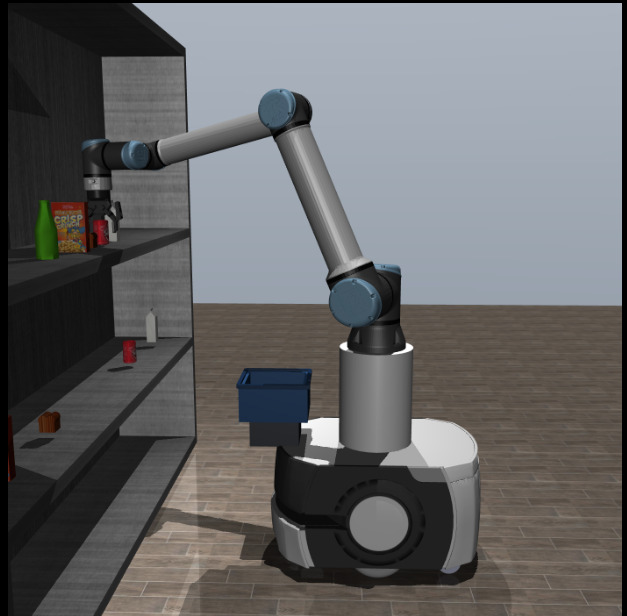
\includegraphics[width=0.75\textwidth,
    alt={The simulated mobile manipulator: an Omron mobile base with a UR10e arm and gripper, facing a stocked supermarket shelf, with a basket mounted on the base.}]{figures/image.jpeg}
\end{center}
\caption{The simulated supermarket workspace: an Omron mobile base carrying a
UR10e arm and Robotiq gripper, a stocked shelf of textured grocery meshes, and an
onboard basket as the drop target.}
\label{fig:system}
\end{figure}

\begin{figure}[ht]
\begin{center}
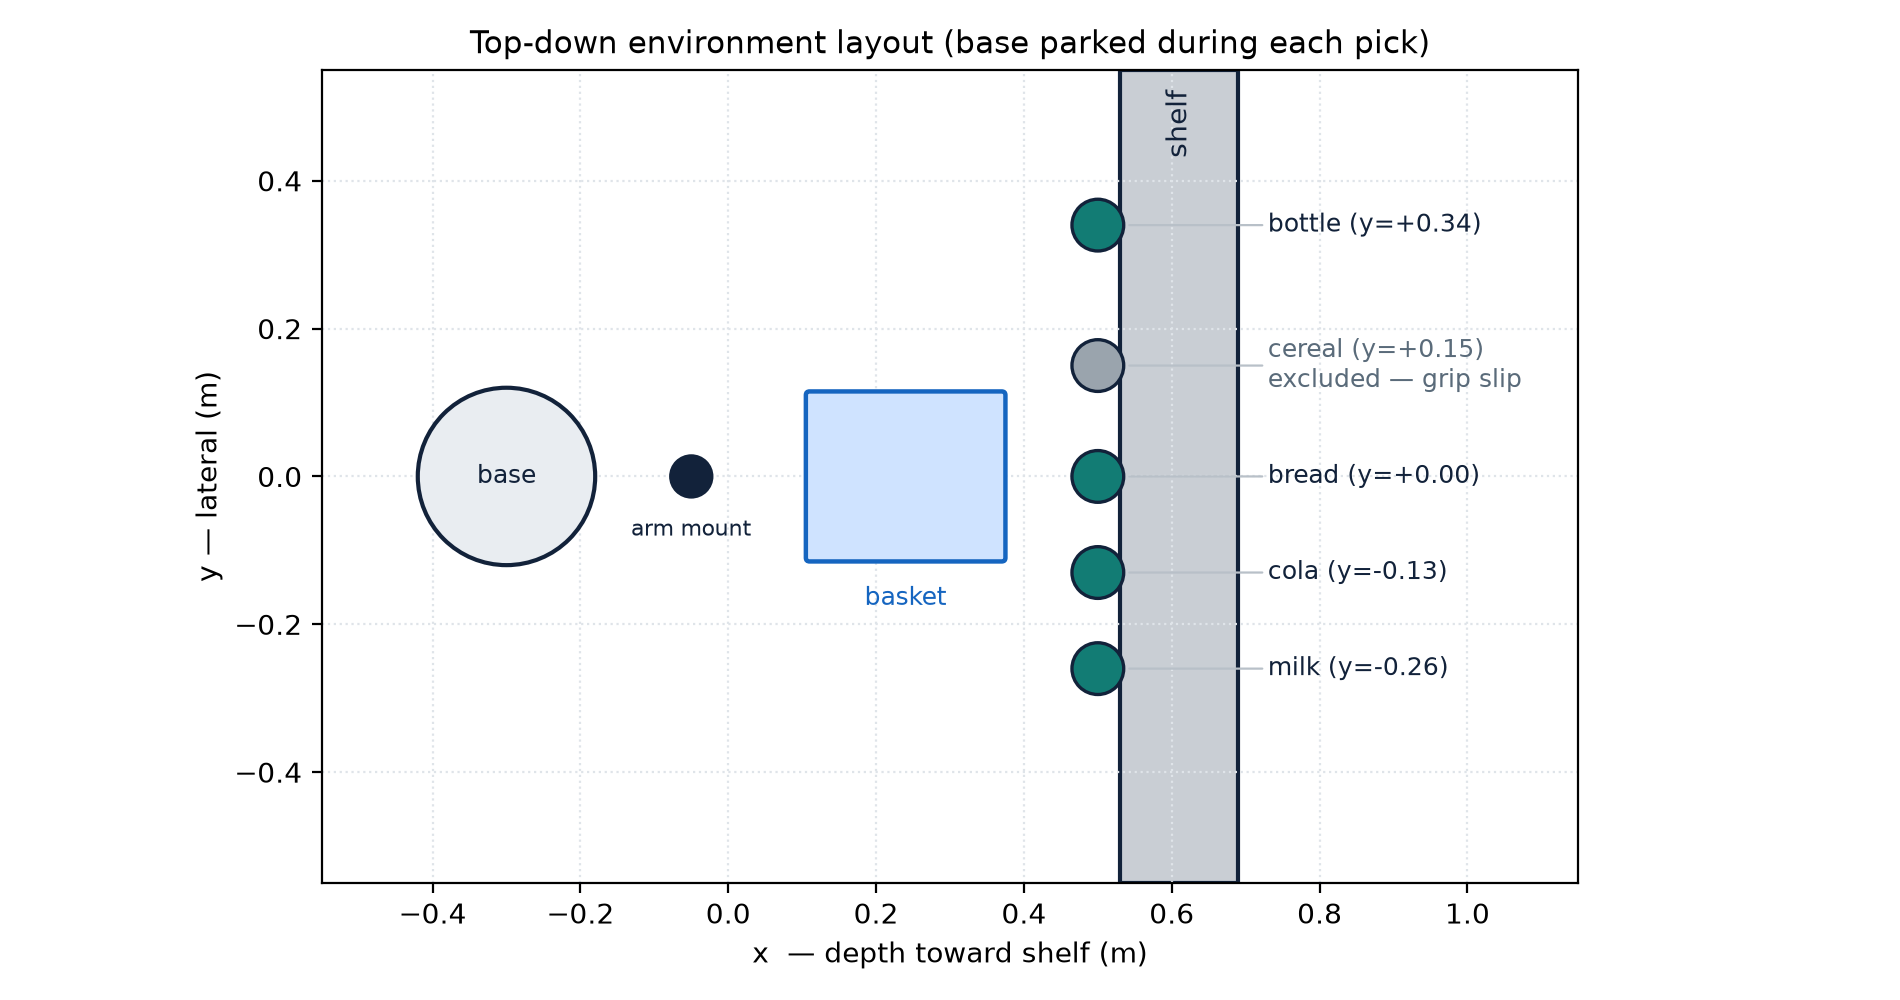
\includegraphics[width=0.85\textwidth,
    alt={A top-down schematic of the environment showing the parked base, the arm mount, the basket on the deck, and the five grocery items along the shelf front at their lateral positions.}]{figures/fig_env_layout}
\end{center}
\caption{Top-down schematic of the task geometry (metres, base frame). Products
rest along the shelf front at the indicated lateral positions, all at $x=0.880$; the
cereal box is shown for completeness but is excluded from training and from all
reported results, as it slips in the two-finger gripper. Note that the water bottle
($y=+0.34$), not the milk carton ($y=-0.26$), is the most laterally displaced item.}
\label{fig:layout}
\end{figure}

\subsection{Arm, gripper and workspace}
\label{sec:m-arm}
The UR10e is a six-degree-of-freedom serial manipulator with a nominal reach of
approximately \SI{1.3}{m} and a spherical wrist, which gives a large, dexterous
workspace well suited to reaching across a shelf and over the basket. The six
revolute joints are driven by MuJoCo position servos; commanding a joint
configuration and stepping the physics under gravity compensation causes the arm to
converge to that configuration. Because the arm is redundant for a purely positional
grasp target only in orientation (six joints for a six-dimensional pose), the
inverse-kinematics problem is well posed but sensitive to the branch of the solution,
which motivates the home-seeding described in \refsec{sec:m-ik}.

The Robotiq 2F-85 is an under-actuated parallel gripper with an \SI{85}{mm} stroke,
modelled with the tendon-driven finger coupling from the MuJoCo Menagerie. Its single
control input is mapped to a normalised opening in $[0,1]$, which is the seventh
dimension of both the state and the action. Because the fingers are rigid and the
robosuite meshes are smooth, a friction-only grip is prone to slipping during the
accelerations of transport; this is countered by enabling additional no-slip solver
iterations while the item is held and by keeping transport motions gentle, and the
no-slip iterations are disabled at the instant of release so the item falls freely
into the tote rather than being flung.

The policy observes the scene through three cameras, illustrated in
\reffig{fig:cameras}: a \emph{wrist} camera (eye-in-hand, \SI{75}{\degree} field of
view) for the close-up grasp; a \emph{scene} camera facing the shelf for object
localisation; and a \emph{basket} camera aimed at the drop target. The basket camera
was not part of the original design: it was added in response to the failure analysis
of \refsec{sec:results-diagnosis}, where poor observability of the drop target was
identified as a cause of the initial placement failures. It is described here with the
rest of the final configuration for coherence. Each camera is rendered at
$96\times96$ pixels. These three images, together with the arm's
seven-dimensional proprioceptive state and the text instruction, constitute the
entire input to the policy; crucially, \emph{no object coordinates or segmentation
are provided}, so any localisation of the named item must be derived from pixels. It
should be noted at the outset --- and is established in \refsec{sec:results-lookup} ---
that withholding object coordinates does not by itself compel the policy to localise:
because each item occupies a fixed position throughout the demonstrations, associating
the item word with a memorised trajectory also fits the data, and that is what the
trained policy is found to do.

\begin{figure}[ht]
\begin{center}
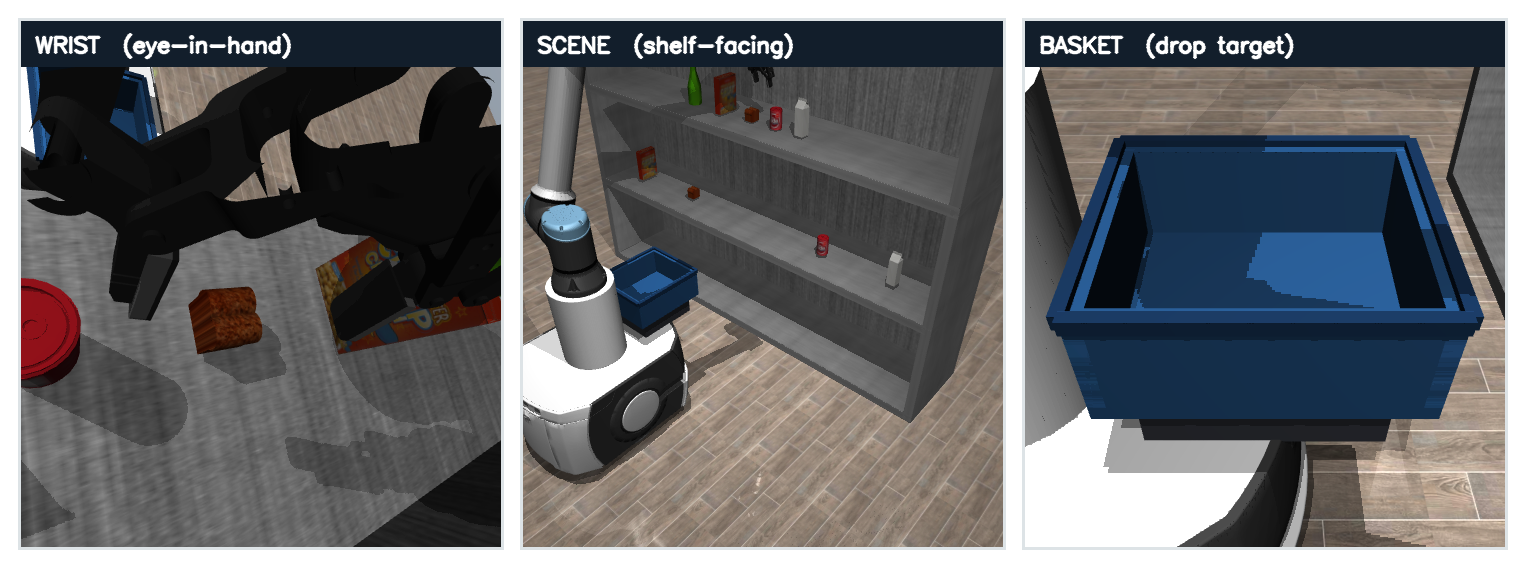
\includegraphics[width=\textwidth,
    alt={Three camera views: a wrist eye-in-hand view of the gripper, a scene view of the shelf, and a basket view of the drop target.}]{figures/camera_views}
\end{center}
\caption{The three synchronised camera views the policy receives every step:
wrist (eye-in-hand), scene (shelf-facing) and basket (drop target).}
\label{fig:cameras}
\end{figure}

\subsection{Rendering and image preprocessing}
\label{sec:m-render}
Camera frames are produced by MuJoCo's off-screen renderer through EGL, which allows
data generation and evaluation to run without a display --- essential for headless,
scripted collection of hundreds of episodes. Each camera renders an RGB image that is
resized to $96\times96$ before being passed to the policy. This modest resolution is a
deliberate compromise: it is large enough to localise the products and read the drop
target, but small enough that three streams can be encoded by the backbone within the
memory budget and at an interactive rate. At both training and inference the images
pass through the policy's pre-processor, which normalises pixel values and arranges the
channels as the backbone expects; the same pre-processor is used in both phases, so the
policy never sees an image distribution at test time that differs from training. The
live interactive viewer used for qualitative inspection renders through a display
rather than EGL and is used only for visualisation, not for measured results.

\section{Scripted expert and inverse kinematics}
\label{sec:m-expert}

\subsection{Differential inverse kinematics}
\label{sec:m-ik}
Grasp and place poses are solved with \texttt{mink} \parencite{zakka2024mink}, a
MuJoCo-native differential inverse-kinematics library. At each solver iteration the joint velocity
$\dot{\mathbf{q}}$ is obtained by solving a small quadratic program that minimises
the weighted end-effector task error subject to kinematic limits,
\begin{equation}
\min_{\dot{\mathbf{q}}}\;
\sum_{k} \big\lVert \mathbf{J}_k \dot{\mathbf{q}} - \mathbf{v}_k^{\star} \big\rVert^2
\quad\text{s.t.}\quad
\dot{\mathbf{q}}_{\min} \le \dot{\mathbf{q}} \le \dot{\mathbf{q}}_{\max},
\label{eq:ik}
\end{equation}
where $\mathbf{J}_k$ is the task Jacobian and $\mathbf{v}_k^\star$ the desired task
velocity for task $k$ (end-effector position and orientation). The mobile base is
pinned by a velocity limit and the arm respects a configuration limit, so only the
six arm joints move. Because \eqref{eq:ik} is solved iteratively from the current
configuration, it is a \emph{local} solver: grasp IK is therefore seeded from the
arm's actual home configuration, which yields a solution on the same kinematic
branch that the position servos can subsequently track. Seeding from an arbitrary
pose was found to produce joint solutions that wrap beyond $\pm 2\pi$ or that the
servo cannot follow, causing the gripper to close off-centre.

\subsection{Pick-and-place trajectory}
\label{sec:m-traj}
Because the target shelf bay is boxed in from above, the item cannot simply be
lifted vertically clear of the shelf. Instead the expert executes a top-down grasp
followed by a \emph{frontal extraction}: the grasped item is pulled straight out of
the shelf front at grasp height before being carried to the basket. The full phase
sequence is listed in \reftab{tab:phases}. Grip stability on the smooth robosuite
meshes is maintained by enabling no-slip solver iterations during transport; these
are disabled immediately before release so the item drops cleanly into the tote.

\begin{table}[ht]
\caption{Phases of the scripted pick-and-place trajectory. Interpolation steps are
executed under the arm position servos, stepping the physics between waypoints.}
\begin{center}
\tagpdfsetup{table/header-rows={1}}
\begin{tabular}{lll}
\toprule
Phase & Gripper & Purpose \\
\midrule
Home              & open          & settle at the trained start pose \\
Pre-grasp         & open          & position above the item \\
Grasp             & open          & descend to grasp height \\
Close             & open$\to$closed & secure the item \\
Lift              & closed        & raise into the opened shelf bay \\
Extract           & closed        & pull straight out of the shelf front \\
Approach          & closed        & move over the basket \\
Lower / place     & closed        & descend over the tote \\
Release           & closed$\to$open & drop the item (no-slip disabled) \\
Settle            & open          & hold while the item settles \\
\bottomrule
\end{tabular}
\end{center}
\label{tab:phases}
\end{table}

\subsection{Per-item grasp tuning}
\label{sec:m-grasp}
Reliable grasping required per-item parameters, summarised in
\reftab{tab:grasptune}: the finger-closing yaw, the grip height (wrist-to-item
offset) and the item's rest position. The cereal box, being the widest item,
requires the fingers to close across its narrow face; the water bottle, being
tall, requires a higher grip point for a stable hold; and the milk carton was
moved inward from the reach edge to prevent it toppling under jitter. With these
tunings the expert succeeds, under per-episode jitter, on the four retained items
with rates of 100\% (cola), 100\% (bread), 98\% (milk) and 96\% (bottle). The
cereal box is excluded from training: even with a $90^\circ$ grasp yaw it slips in
transport, and reliably teaching a policy from unreliable demonstrations is not
possible.

\begin{table}[ht]
\caption{Per-item grasp parameters and scripted-expert success rate (with
per-episode positional jitter).}
\begin{center}
\tagpdfsetup{table/header-rows={1}}
\begin{tabular}{lccc}
\toprule
Item & Grasp yaw & Notable tuning & Expert success \\
\midrule
Cola can     & default & ---                         & 100\% \\
Bread loaf   & default & ---                         & 100\% \\
Milk carton  & default & moved inward from reach edge & 98\% \\
Water bottle & default & higher grip point           & 96\% \\
Cereal box   & $90^\circ$ & \emph{excluded} (grip slip) & --- \\
\bottomrule
\end{tabular}
\end{center}
\label{tab:grasptune}
\end{table}

\section{Demonstration collection and dataset}
\label{sec:m-data}
For each successful episode, the recorder stores, per control step: the three
camera images ($96\times96$), the seven-dimensional state (six arm joint angles and
the gripper opening), the seven-dimensional action (the executed servo command),
and a natural-language instruction. To make the policy \emph{language-conditioned}
rather than reliant on a single memorised sentence, the instruction is drawn from a
set of six paraphrase templates (for example, ``pick up the
\{item\} and place it in the basket'', ``grab the \{item\} and put it in the
basket''), with one template sampled per episode. The identical template module is
used at inference to guarantee train--deploy consistency. Each item's planar
position is randomly jittered by up to \SI{2.5}{cm} per episode, and the grasp IK is
re-solved on the settled position so that the demonstrations cover a distribution
of grasp poses rather than a single canonical trajectory.

Only \emph{successful} demonstrations are retained. Success is verified physically at
the end of each scripted episode by checking that the target item has come to rest
inside the basket footprint and low (not perched on the rim), using the same
geometric criterion later applied to the learned policy; episodes that fail this check
are discarded rather than saved. This guards against a subtle failure mode observed in
the pilot study, where an over-permissive success check admitted demonstrations in
which the item was merely near the basket, teaching the policy an imprecise notion of
``placed''. Verifying demonstrations with the same metric used for evaluation keeps
the definition of success consistent across data collection, training and testing.

A design choice that proved decisive concerns the \emph{episode boundary}:
demonstrations end at the instant of placement. The return-to-home motion is a
reset for the next episode rather than part of the demonstration, and recording it
in an earlier iteration taught the policy to move away immediately after releasing,
knocking the item back out of the basket (\refsec{sec:results-diagnosis}).

In total, 240 successful demonstrations were collected (60 per item across the four
retained items) and converted to the LeRobot dataset format (parquet plus encoded
video) \parencite{cadene2024lerobot}. Of these, \textbf{208 were used for training and 32
(8 per item) held out for validation}; all results reported in \refChap{chap:results}
therefore rest on 208 training demonstrations. The \SI{100}{Hz} recordings are subsampled by a
factor of five to \SI{20}{fps}, so that a fixed-length action chunk spans a useful
temporal horizon rather than a fraction of a second, and a per-item hold-out is
reserved for validation. Normalisation statistics are computed on the training
split and, critically, are frozen with the checkpoint (\refsec{sec:m-eval}).
\reffig{fig:dataset} shows a sample of the recorded streams.

\begin{figure}[ht]
\begin{center}
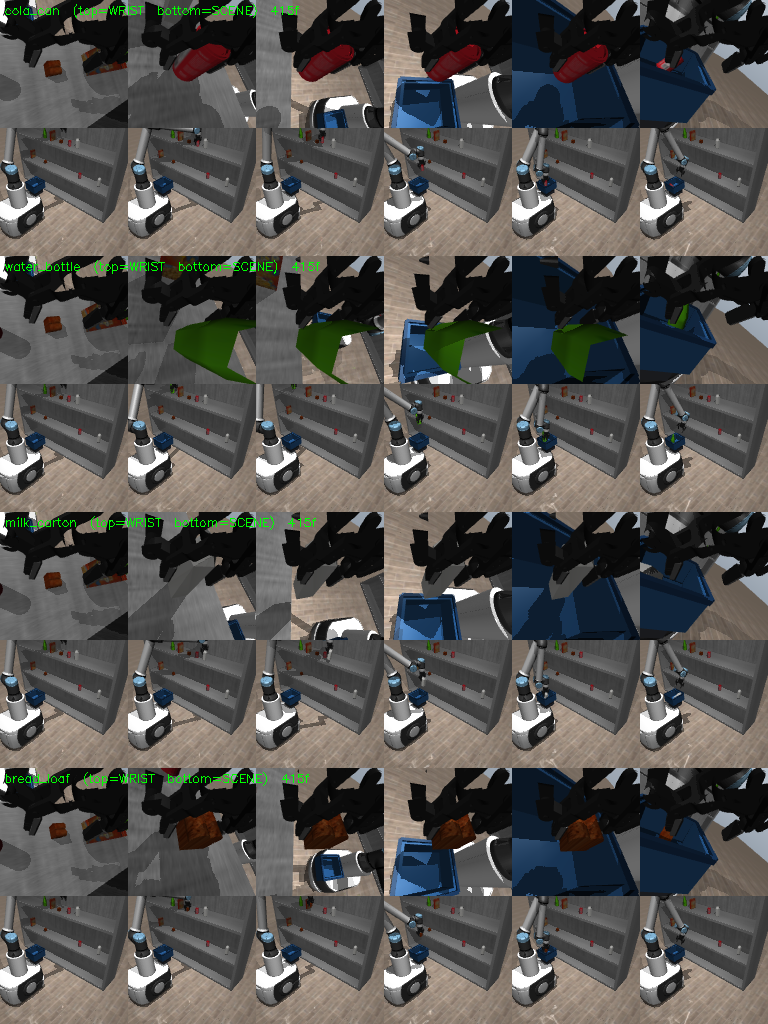
\includegraphics[width=\textwidth,
    alt={A filmstrip of recorded demonstration frames showing the wrist and scene camera streams across a pick-and-place for each item.}]{figures/dataset_preview}
\end{center}
\caption{A sample of the demonstration dataset: wrist and scene camera streams
across a pick-and-place, for each of the four training items. This sample predates
the addition of the basket camera (\refsec{sec:results-diagnosis}); the deployed
configuration records three streams per step.}
\label{fig:dataset}
\end{figure}

\reffig{fig:pickplace} shows key frames of the scripted trajectory that generates
these demonstrations.

\begin{figure}[ht]
\begin{center}
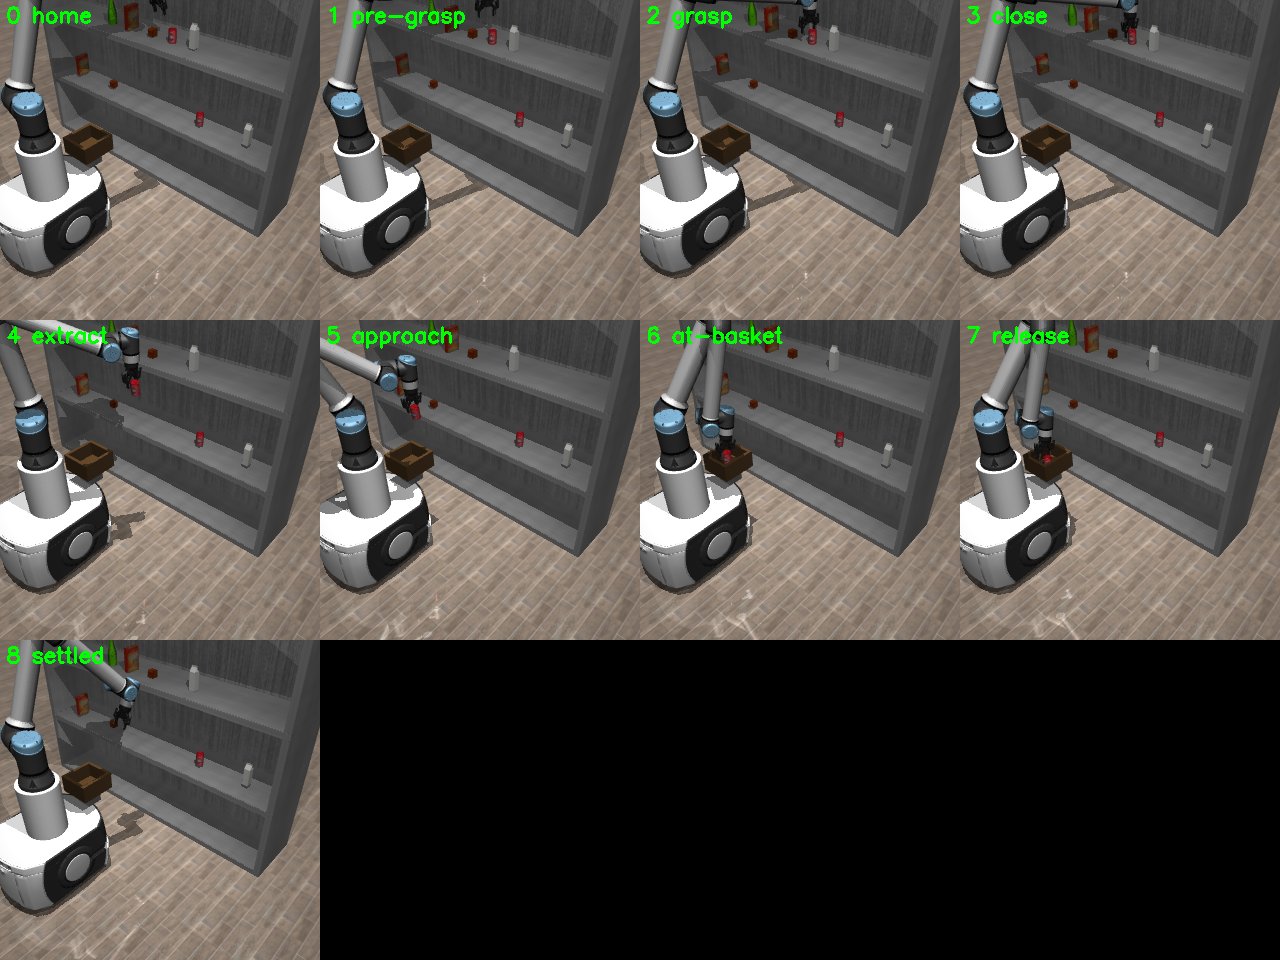
\includegraphics[width=\textwidth,
    alt={A filmstrip of the scripted pick-and-place: home, pre-grasp, grasp, lift, extract, carry over the basket, and place.}]{figures/pickplace_cola_can}
\end{center}
\caption{Key frames of the scripted-expert pick-and-place used to generate
demonstrations, from home pose through grasp, extraction and placement.}
\label{fig:pickplace}
\end{figure}

\subsection{Instruction generation and language conditioning}
\label{sec:m-lang}
Each demonstration is labelled with a natural-language instruction sampled, at
collection time, from a small library of paraphrase templates parameterised by the
item name --- for example ``pick up the \{item\}\ and place it in the basket'', ``grab
the \{item\}\ and put it in the basket'', ``take the \{item\}\ and drop it in the
basket''. Six templates across the four retained items yield 24 distinct
instructions in total (the full list is given in Appendix~\ref{app:Implementation}). The
purpose of this variety is to prevent the policy from binding to one exact sentence:
if every ``milk'' episode used identical wording, the model could in principle key on
the surface form rather than on the meaning. Paraphrasing forces the language signal
that survives across templates --- the item identity --- to be the informative one,
which is what a pretrained vision--language backbone is well placed to extract. The
identical template module is imported by both the data-collection and the inference
code, so the distribution of instructions seen at test time matches that seen during
training; this train--deploy consistency is a small but important guard against an
accidental mismatch that would degrade grounding. At inference the instruction is
tokenised and passed to the backbone alongside the images, exactly as during training.

\subsection{Observation and action spaces and the control loop}
\label{sec:m-spaces}
The observation supplied to the policy at each decision is the tuple
$(\mathbf{I}_{\text{wrist}}, \mathbf{I}_{\text{scene}}, \mathbf{I}_{\text{basket}},
\mathbf{s}, \ell)$, where each image $\mathbf{I}$ is a $96\times96$ RGB frame,
$\mathbf{s}\in\mathbb{R}^{7}$ is the proprioceptive state (six arm joint angles and
the gripper opening, the latter normalised to $[0,1]$), and $\ell$ is the tokenised
language instruction. The action $\mathbf{a}\in\mathbb{R}^{7}$ comprises six
absolute arm-joint targets and a gripper command in $[0,1]$; the policy predicts a
chunk of fifty such actions per forward pass.

The closed-loop control cycle proceeds as follows. The current observation is
assembled and passed through the pre-processor (which applies the frozen
normalisation statistics); the policy predicts a fifty-step action chunk; the chunk
is de-normalised by the post-processor; and its actions are applied to the arm
position servos and the gripper actuator, with the physics stepped exactly
twenty-five substeps per action (approximately \SI{20}{Hz}) before the next action.
When the chunk is exhausted the policy re-plans from the new observation. This
matches the horizon at which the demonstrations were sub-sampled, so that the action
chunk the policy learns to produce spans a comparable slice of real time. Between
consecutive items in a multi-item episode the arm is returned to its home
configuration (the same start state as during data collection) so that each pick
begins in-distribution; the scene itself is not reset, so previously collected items
remain in the basket.

\section{Fine-tuning SmolVLA}
\label{sec:m-train}
The policy is fine-tuned from the pretrained \texttt{smolvla\_base} checkpoint. The
architecture and the training split are summarised in \reffig{fig:architecture}.
SmolVLA couples a compact vision--language backbone (SmolVLM-2) with a
flow-matching action expert that predicts a chunk of future actions
\parencite{shukor2025smolvla, kiviranta2025smolvla}. The backbone tokenises the three
images and the instruction and, through interleaved cross- and self-attention,
produces a fused representation; SmolVLA additionally reduces the number of visual
tokens and lets the action expert read features from an intermediate backbone layer,
both of which lower inference cost \parencite{shukor2025smolvla}.

The action expert is trained by a \emph{conditional flow-matching} objective. Let
$\mathbf{a}_1$ denote a demonstrated action chunk and $\mathbf{a}_0\sim\mathcal{N}
(\mathbf{0},\mathbf{I})$ a noise sample; along the linear path
$\mathbf{a}_\tau=(1-\tau)\mathbf{a}_0+\tau\mathbf{a}_1$ for $\tau\in[0,1]$ the target
velocity is $\mathbf{a}_1-\mathbf{a}_0$. The network $v_\theta$ regresses this
velocity conditioned on the backbone features $\mathbf{c}$ and the proprioceptive
state,
\begin{equation}
\mathcal{L}(\theta)=\mathbb{E}_{\tau,\mathbf{a}_0,\mathbf{a}_1}
\big\lVert v_\theta(\mathbf{a}_\tau,\tau,\mathbf{c})-(\mathbf{a}_1-\mathbf{a}_0)\big\rVert^2 .
\label{eq:flow}
\end{equation}
At inference the learned field is integrated from a noise sample over a small number
of steps to produce an action chunk. Two properties of \eqref{eq:flow} matter here:
actions are continuous, which suits smooth manipulation; and sampling is
\emph{stochastic}, so repeated queries on the same observation give slightly
different chunks --- which is why success is a distribution to be estimated over many
trials rather than a fixed value (\refsec{sec:m-stats}).

\begin{figure}[ht]
\begin{center}
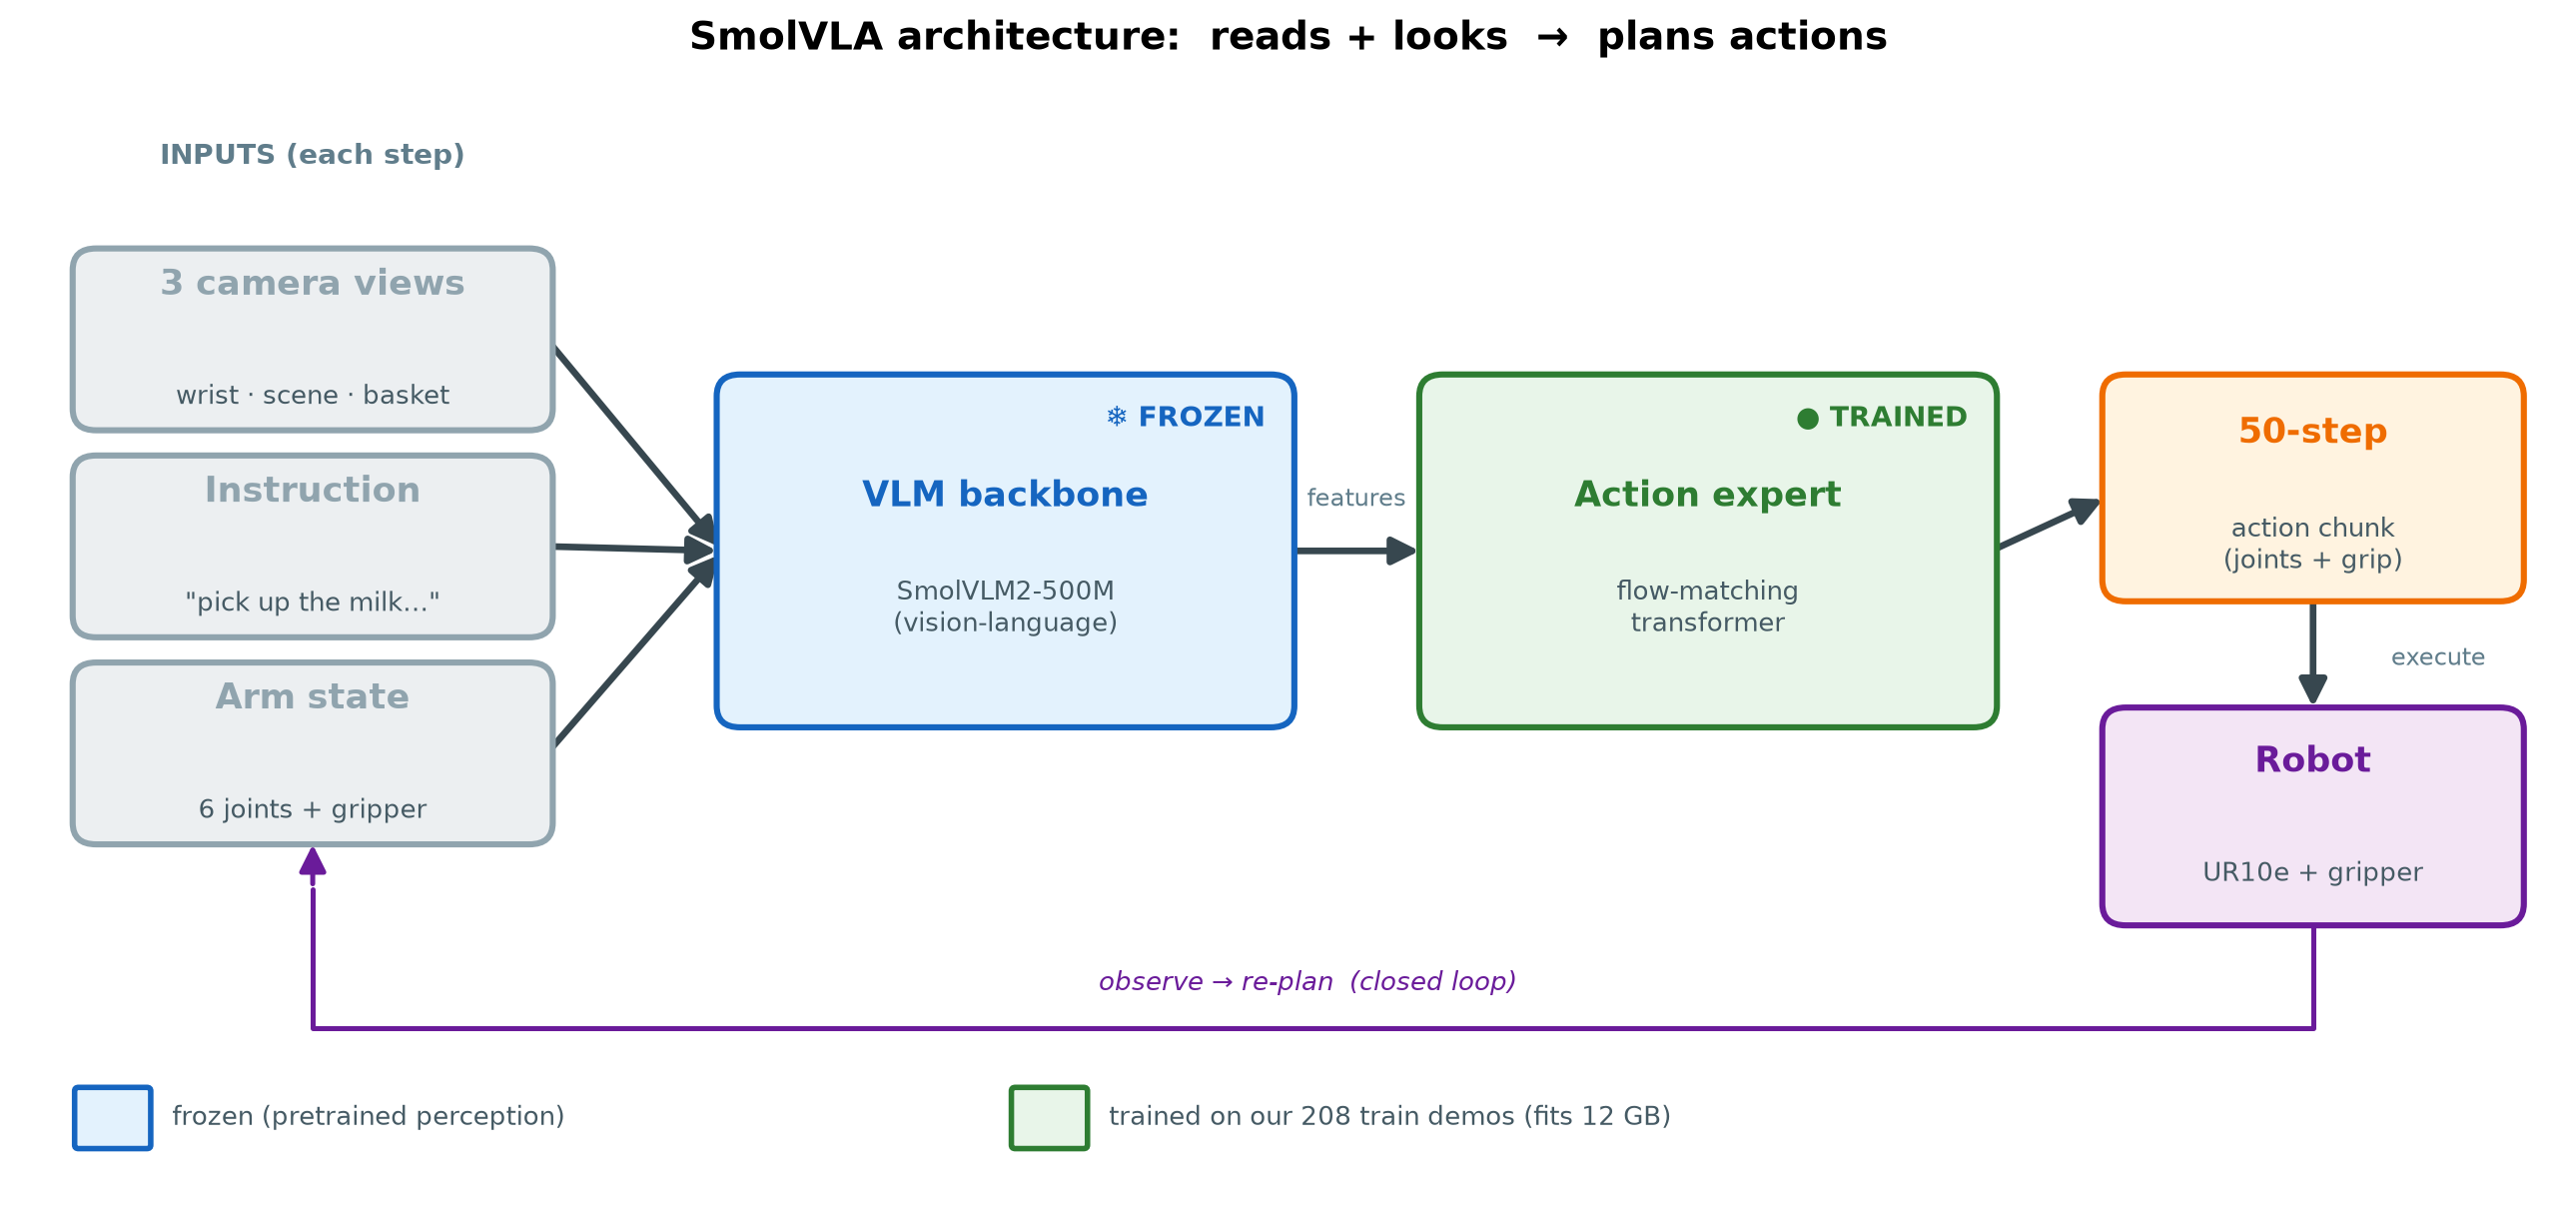
\includegraphics[width=\textwidth,
    alt={A block diagram of SmolVLA: three camera images, the instruction and the arm state feed a frozen vision-language backbone, whose features feed a trained flow-matching action expert that outputs a 50-step action chunk to the robot, in a closed loop.}]{figures/smolvla_architecture}
\end{center}
\caption{SmolVLA architecture and the training split used here. The pretrained
vision--language backbone (frozen) encodes the images and instruction; the action
expert (trained) maps its features and the arm state to a 50-step action chunk,
which is executed before re-planning.}
\label{fig:architecture}
\end{figure}

The decision that makes training feasible within \SI{12}{GB} is to \emph{freeze the
vision--language backbone} and train only the action expert. The rationale is
twofold. First, the backbone was pretrained on large image--text and robot corpora
and already provides strong perception and language grounding; back-propagating
into its roughly 400~million parameters from only 208 training demonstrations would risk
overfitting and catastrophic forgetting of that prior
\parencite{xiang2026posttraining, kiviranta2025smolvla}. In effect, the model already
knows what the objects are and what the words mean, so fine-tuning need only learn
the motor mapping for this specific embodiment. Second, freezing avoids storing
activations for a backward pass through the backbone: the frozen configuration
trains in approximately \SI{3}{GB}, whereas even partially unfreezing the vision
encoder alongside three camera streams exceeded the budget in the preliminary study
(\refsec{sec:results-journey}).

Training uses a batch size of eight for 20{,}000 optimisation steps: each step
draws eight (observation, action-chunk) samples, computes the flow-matching loss,
averages the gradient over the eight, and applies one update. Averaging over a
mini-batch reduces gradient variance relative to a single sample while remaining
within memory; eight was the largest batch that fit comfortably. Training takes
approximately four hours on an NVIDIA RTX~A2000 (\SI{12}{GB}). A checkpoint is
saved every 5{,}000 steps, yielding four candidate snapshots (5k, 10k, 15k and 20k
steps) for the selection procedure below. Complete hyper-parameters are listed in
Appendix~\ref{app:Implementation}.

\section{Experimental design}
\label{sec:m-experiments}
The preceding sections describe how the artefact is built; this one specifies what is
done with it. The measurement procedure itself follows in \refsec{sec:m-eval}.

\subsection{Variables}
\label{sec:m-variables}
Across the experiments, the following are \emph{manipulated} one at a time:

\begin{itemize}
    \item \textbf{Policy architecture} --- SmolVLA (450\,M, language-conditioned)
    versus ACT (52\,M, no language input), trained on identical data (E8).
    \item \textbf{Training checkpoint} --- the four snapshots at 5k, 10k, 15k and
    20k optimisation steps (E3).
    \item \textbf{Instruction} --- which item the text names, with the scene held
    fixed (E5).
    \item \textbf{Object position} --- items moved to lateral positions not used in
    training, or exchanged with one another (E6).
    \item \textbf{Evaluation protocol} --- object pose fixed at its nominal value
    versus jittered by up to \SI{2.5}{cm}, the same jitter used at collection time (E7).
    \item \textbf{Observation and data configuration} --- the presence of the basket
    camera, the episode boundary, and the tote footprint (E4).
    \item \textbf{Task length} --- single-item picks versus shopping lists of two or
    three items (E10).
\end{itemize}

Two outcomes are \emph{measured} per trial, both binary and defined exactly in
\refsec{sec:m-eval}: \emph{grasp success} and \emph{task completion}. Where the
question concerns \emph{where} the arm went rather than whether it succeeded, a third,
continuous measurement is taken --- the gripper's lateral ($y$) position at gripper
closure, compared against both the item's actual position and the position it occupied
during training (E5, E6).

\emph{Held constant} across every comparison, unless under test: the environment model
and physics parameters; camera placements, resolutions and pre-processing; observation
and action spaces; control rate and substeps; training dataset, optimiser and step
budget; the trial seeds; and the evaluation harness itself, a single code path used for
all conditions. Normalisation statistics are loaded from the checkpoint under test, so a
checkpoint comparison cannot be contaminated by a train--deploy mismatch.

Two nuisance sources are managed rather than eliminated: the flow-matching sampler's
stochasticity (\refsec{sec:bg-flow}), handled by estimating success over many trials;
and the instruction paraphrase, drawn afresh per trial. The latter is deliberate --- a
policy working for only one phrasing should not score as instruction-following --- but
per-trial variance therefore includes a language component.

\subsection{Catalogue of experiments}
\label{sec:m-catalogue}
\reftab{tab:experiments} lists every experiment with its manipulated variable, sample
size and purpose. E1 and E2 belong to Phases~1 and~2 (\refsec{sec:m-phases}); E3
onwards are the main study.

\begin{table}[ht]
\caption{Catalogue of experiments. $n$ counts closed-loop rollouts unless otherwise
stated. Identifiers are used in \reftab{tab:rqmap} and in \refChap{chap:results}.}
\begin{center}
\tagpdfsetup{table/header-rows={1}}
\begin{tabular}{p{0.04\textwidth}p{0.26\textwidth}p{0.20\textwidth}p{0.13\textwidth}p{0.10\textwidth}}
\toprule
ID & Experiment & Manipulated variable & $n$ & RQ \\
\midrule
E1 & RoboCasa benchmark feasibility &
Policy (SmolVLA, ACT); GR00T zero-shot as reference &
20 per policy & RQ2 \\
\addlinespace
E2 & Fixed-base UR10e pilot &
Policy (SmolVLA, ACT) $\times$ 5 cube positions &
per \refsec{sec:results-journey} & RQ2 \\
\addlinespace
E3 & Checkpoint sweep and headline result &
Checkpoint (5k/10k/15k/20k) $\times$ item &
320 & RQ1 \\
\addlinespace
E4 & Failure diagnosis and targeted fixes &
Episode boundary, basket camera, tote footprint &
12 (baseline) + single-episode trace & RQ4 \\
\addlinespace
E5 & Language grounding, scene fixed &
Instruction only &
3 instructions & RQ3 \\
\addlinespace
E6 & Displacement and swap &
Object position (4 unseen positions; pairwise swap) &
264 (48 baseline, 216 displaced) & RQ3, RQ4 \\
\addlinespace
E7 & Robustness to object pose &
Evaluation protocol (fixed pose vs.\ \SI{2.5}{cm} jitter) &
320 + 80 control & RQ1, RQ3 \\
\addlinespace
E8 & Same-task capacity control &
Policy (SmolVLA vs.\ ACT); ACT trained on one item vs.\ four &
200 & RQ2 \\
\addlinespace
E9 & Interpretability readout &
--- (observational) &
qualitative & --- \\
\addlinespace
E10 & Multi-item orchestrator &
List length (two, three items) &
40 lists / 100 picks & RQ1 \\
\bottomrule
\end{tabular}
\end{center}
\label{tab:experiments}
\end{table}

\subsection{Sample sizes and their limits}
\label{sec:m-power}
Sample sizes were chosen for the precision they buy. Each configuration is evaluated
over at least twenty trials per item, giving $n\ge 80$ across the four retained items.
At $n=80$ and a rate near 80\%, the Wilson 95\% interval is about $\pm 9$ percentage
points (\refsec{sec:m-stats}) --- narrow enough to distinguish a working policy from a
failing one and to state the headline result with an honest bound.

It is not narrow enough to resolve small differences, and this is stated in advance
rather than discovered afterwards. A five-point gap between checkpoints at $n=80$ is
well inside sampling noise, so \refsec{sec:results-checkpoint} identifies the best
snapshot for deployment rather than claiming significance. Detecting such a difference
would need several hundred trials per checkpoint --- judged a poorer use of compute than
the additional \emph{conditions} in \reftab{tab:experiments}, which proved far more
informative about what the policy had learned. Where a sample is genuinely small this is
not disguised: the 0\% baseline of E4 rests on twelve trials and is reported with its
interval (roughly 0--24\%).

\section{Evaluation methodology}
\label{sec:m-eval}
Policies are evaluated \emph{closed-loop}. The trained policy observes the three
cameras, the arm state and the instruction; it predicts a 50-step action chunk,
which is applied to the environment at approximately \SI{20}{Hz} before
re-planning, until the episode terminates. Two binary outcomes are recorded per
trial: \emph{grasp success} (the item is lifted clear of the shelf at some point in
the episode) and \emph{task completion} (the item comes to rest inside the basket
footprint and low, i.e.\ not perched on the rim), the latter being the headline
metric.

\subsection{Statistical reporting}
\label{sec:m-stats}
To avoid over-reading small samples, each configuration is evaluated over at least
twenty trials per item ($\ge 80$ in total), with a fresh random seed and a freshly
sampled instruction paraphrase per trial, and results are reported with
\emph{Wilson} score 95\% confidence intervals \parencite{wilson1927ci}. For $k$
successes in $n$ trials with $\hat{p}=k/n$ and $z=1.96$, the interval is
\begin{equation}
\frac{1}{1+\frac{z^2}{n}}
\left(
\hat{p}+\frac{z^2}{2n}
\;\pm\;
z\sqrt{\frac{\hat{p}(1-\hat{p})}{n}+\frac{z^2}{4n^2}}
\right).
\label{eq:wilson}
\end{equation}
The Wilson interval is preferred over the normal approximation because it remains
within $[0,1]$ and behaves sensibly for proportions near the boundaries and for
modest $n$ --- both relevant here, where item rates range from 60\% to 100\% at
$n=20$. \textcite{brown2001binomial} recommend it for precisely this regime.

The analysis plan for \emph{comparisons} is declared here rather than chosen after
seeing the data. Because configurations are evaluated on the same trial seeds, the
observations are paired, and the appropriate test is McNemar's exact test on the
discordant pairs \parencite{mcnemar1947test} rather than a two-sample test on the
marginal rates. Across several comparisons in one family --- the six pairs among four
checkpoints --- the family-wise error rate is controlled by Holm's sequentially
rejective procedure \parencite{holm1979correction}, uniformly more powerful than
Bonferroni at the same guarantee. Both uncorrected and corrected $p$-values are
reported.

Two consequences follow. The plan will frequently return a null at these sample sizes
(\refsec{sec:m-power}), and a null is reported as such. And the deployment decision and
the significance test answer different questions: the deployed checkpoint is the one
with the highest measured task completion, which remains the right operational choice
even where the difference is not significant.

\subsection{Checkpoint selection}
\label{sec:m-checkpoint}
The deployed checkpoint is selected by \emph{closed-loop task success rather than
by training or validation loss}. All four saved snapshots are evaluated over eighty
trials each, and the checkpoint with the highest task-completion rate is chosen. To
prevent a train--deploy mismatch, the pre- and post-processing normalisation
statistics are loaded from the same checkpoint, so that the actions the policy
emits are unnormalised with exactly the statistics under which it was trained.
\refsec{sec:results-checkpoint} shows that this choice is not academic: the final
checkpoint is not the best.

\section{Ethics and research-data management}
\label{sec:m-ethics}
The study involves no human participants, no personal data and no animal subjects. All
experiments are in simulation, so there is no risk of physical harm and no machinery
safety case is required. Ethical approval was nonetheless sought and granted through
the University's CURES process; the letter is reproduced in
Appendix~\ref{app:EthicalApproval}.

All third-party components are open source and used within their licences: MuJoCo and
the Menagerie \parencite{todorov2012mujoco, deepmind2022menagerie}, robosuite assets
\parencite{zhu2020robosuite}, LeRobot \parencite{cadene2024lerobot}, \texttt{mink}
\parencite{zakka2024mink} and the \texttt{smolvla\_base} checkpoint
\parencite{shukor2025smolvla}. The dataset is entirely synthetic and contains no
recorded human behaviour. Datasets, checkpoints, logs and code are retained together so
a reported number can be traced to the rollout that generated it
(Appendix~\ref{app:Implementation}).

One ethical consideration applies to the reporting rather than the conduct. A
language-conditioned system is easy to over-claim: an 80\% success rate at a fixed
object pose could be presented as ``a robot that fetches what you ask for'', which
\refChap{chap:results} shows would misrepresent what the policy does. The commitment
here is to report the conditions under which each number holds alongside it.

\section{Summary}
\label{sec:m-summary}
The methodology rests on five commitments, each tested in \refChap{chap:results}: the
\SI{12}{GB} budget is fixed in advance and every design decision made inside it
(\refsec{sec:m-train}); the pipeline is built incrementally, each stage verified against
a criterion independent of the learned policy (\refsec{sec:m-dev}); success is defined
geometrically and applied identically at collection and evaluation time
(\refsec{sec:m-data}, \refsec{sec:m-eval}); experiments manipulate one variable at a
time against a fixed harness and paired seeds, with sample sizes and their limits
declared in advance (\refsec{sec:m-experiments}); and when a policy underperforms, the
response is to diagnose before scaling (\refsec{sec:m-diagnostic-loop}).
